
\documentclass[11pt,letterpaper,oneside]{article}
\usepackage[top=1in,left=1in,right=1in,bottom=1in]{geometry}
\usepackage{textcomp}
\usepackage{fancyvrb}
\usepackage{colortbl}
\usepackage{graphicx}
\usepackage{url}

\title{coDoc: A Tool for Managing Relationships between Codes and Documents}
\author{Dejun Qian}

\begin{document}
\maketitle

\begin{abstract}
When writing and testing software, 
we need the documents in hand.
This is extremely true for software that is document intensive, 
such as hardware driver and virtual device.
This paper presents coDoc, 
an integrated development environment for managing relationships between codes and documents. 
We first describe the architecture and features of coDoc.
We then discuss several design decisions that we faced in developing coDoc and the trade-offs in making these decisions.
To provide perspective,
we report our experiences in mapping two virtual network interface card (NIC) to the real NIC documents.
\end{abstract}

% Include the motivation for your work, your approach, your goals, and a short summary of what you found/achieved/tested.
\section{Introduction}
\label{sec:introduction}
Documents play an important role in software engineering process,
from requirement analysis to architecture design,
from code written to software testing,
from software maitentence to software updating.
Software that relates closely to hardware devices is extremely document intensive.
Examples of these software could be bootloader, 
Operating System (OS) Hardware Abstraction Layer (HAL),
virtual devices of virtual machines.
These software should conform to hardware documents.
A typical embedded CPU usually have documents with thousands of pages.
A computer system usually is consisted of over ten hardware modules.
To effectively maintain the relationships between the codes and the documents is really important for developing and verification of these software.

Many work has been done to deal with the relationships between Application Programming Interface (API) documents and its client codes \cite{Pandita_inferring_2012}.
API documents are usually well indexed by the functions or the class.
When we are interested in a piece of code in the client software,
we can easily find the related API document by the invoded function.
The relationships between the client codes and the API documents are easily constructed by using the function name as the keyword.
However, the code related to hardware and its documents are usually related in a different way.
The main reason is that the hardware document usually talks about how to use the hardware,
more specifically how to program the registers inside the hardware module.
Different from the API document,
we can not locate the document for a piece of hardware related code, and vice versa,
because there exists no similar keywork like the function name or the class name.

The hardware documents differ from the API documents in the following ways,
\begin{itemize}
\item the hardware documents are usually published as pdf files, while the API documents are usually html files
\item the hardware documents are composed of texts, tables and diagrams, while the API documents are usually texts only
\item hard for the computer to relate the document piece to the code piece automatically
\end{itemize}

These differences make the construction of the relationships between the hardware related codes and their documents really challenging.
To our knowlege, there is no tool exists to address this problem.
People usually write down the position of the related document piece in the document as a comment of the code.
This is a simple workaround as no easier tools are available.
However, this method can only handle simple situations.
If there are thousands of these comments, 
and there are cluttered over in the code,
then it will be very hard to manage.
This paper presents coDoc, a tool to easily create, maintain, and display the relationships.
% The initial version\footnote{\texttt{\url{git@github.com:derekqian/coDoc.git}}} has been released.
The key features of coDoc are as follows,
\begin{itemize}
\item provide the ability to display code and document. 
\item select code based on syntax parsing.
\item stable to the change of unrelated code.
\item make relationship between code and document.
\item display the relationship.
\end{itemize}

Using coDoc, we have created relationships for to virtual NIC devices fo qemu.
These two devices are DIO and E100.

The rest of the paper is orgnized as follows. 
Section \ref{sec:background} introduce the background of poppler and CDT.
Section \ref{sec:arch} provides the overall architecture and key features of coDoc.
Section \ref{sec:decision} gives the design decisions of coDoc and the trade-offs of these decisions.
Section \ref{sec:evaluation} summarizes our experiences of creating and maitaining the relationships for two virtual devices.
Section \ref{sec:related} presents the related work.
Section \ref{sec:conclusion} conclude our work and give some thinking towards the future.


% Explain your design / languages, libraries, and tools used, experimental design.
\section{Background}
\label{sec:background}
\subsection{poppler}
We adopt poppler, a open-source pdf render, to render pdf content in coDoc.
This PDF render is written in C++, 
and is widely used in Linux systems.
It uses Cairo and GTK to draw the rendered content.

\subsection{C Development Tool}
CDT is an Eclipse plugin which supports C/C++ syntax parsing.
It is written in Java and provide Eclipse with the ability of syntax highlighting and code completion when developing C/C++ code.


% This should NOT be raw data or code listings.  Instead you should present the key arch from your work.  Be guided by the papers you have read this quarter - in cases where it is necessary for understanding, a small section of code might be listed, separate from the text, but more commonly an algorithm might be shown.  Result are not long tables of data, rather, one or two graphs, or tables with key rows or columns highlighted or italicized.
\section{Architecture and Features of coDoc}
\label{sec:arch}
The result for the experiment is shown in fig.

\subsection{Build and Make existing code}
On the first stage of our work, we tried to make the software user-friendly. Basically, the following work is done,
\begin{enumerate}
\item Added Makefile and instructions.
\item Added accurate "usage" message to output.
\end{enumerate}

\begin{figure}
\begin{center}
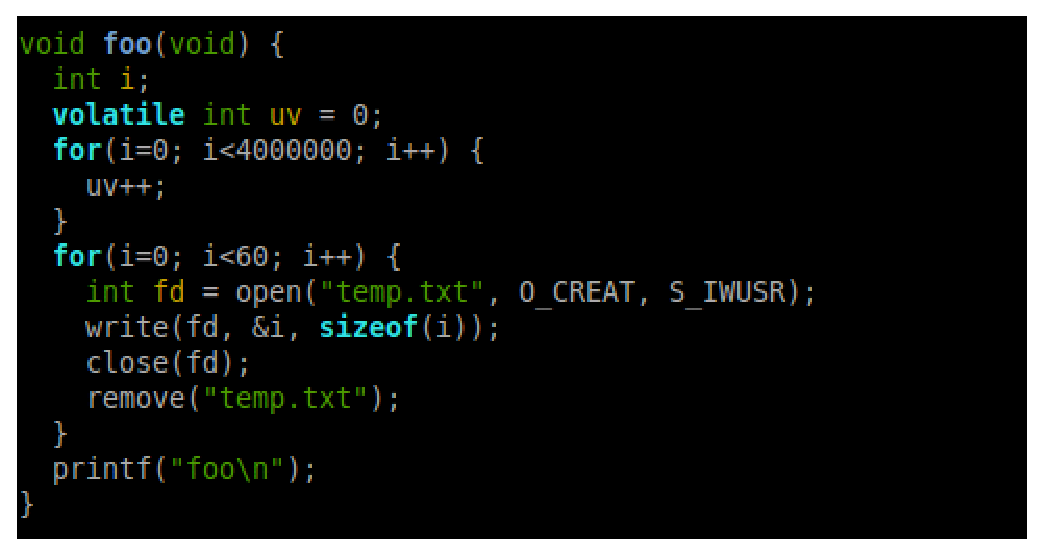
\includegraphics[width=0.6\textwidth]{codoc.eps}
\caption{Structure of Dyninst}
\label{fig:codoc}
\end{center}
\end{figure}

How coDoc works is illustrated in Figure \ref{fig:codoc}\footnote{\texttt{from Bryan's paper \cite{xiao_automated_2012}}}. 
A \emph{point} is a location in a program.

\noindent \newline\textbf{Instrument Using Dyninst}\newline
\indent Figure \ref{fig:codoc} gives a general idea about how coDoc works.

The code used to achieve this goal is shown bellow,
\begin{Verbatim}[frame=single]
printf(``Hello world!'');
\end{Verbatim}


After downloading Elipse\footnote{\texttt{\url{http://www.eclipse.org}}}, we need install JDK.

To test this feature, we designed a test program. 
The functions implemented in the test program is listed in Table \ref{table:functions}.

\begin{table}[th]
\caption{Functions implemented in hello}
\centering
\begin{tabular}{rl}
\hline
Function & Description \\
\hline
fake & functioin never called \\
foo  & basic function \\
recursive & function call itself recursively \\
main & main function \\
\hline
\end{tabular}
\label{table:functions}
\end{table}

\section{Methodology and Design Decisions}
\label{sec:decision}
The result for the experiment is shown in fig.

\section{Evaluation}
\label{sec:evaluation}
The result for the experiment is shown in fig.

\section{Related Work}
\label{sec:related}
The result for the experiment is shown in fig.


% Based on what you have so far, what can you conclude?  What cool ideas did you think up but not have time to implement so far?
\section{Conclusions and Future Work}
\label{sec:conclusion}
There is still a great deal of opportunity to improve coDoc.

One way to construct the relationship for hardware related code and its documents is to use machine learning method.
This method need the seed data to train the model.


% Follow a standard ACM format for your references.  You have examples in the papers you have read.
\bibliographystyle{acm}
\bibliography{reference}

%\begin{thebibliography}{9}
%\bibitem{bib:coDoc}
%\emph{http://www.coDoc.org}
%\end{thebibliography}

\end{document}
